\documentclass[11pt]{article}
\usepackage[letterpaper,margin=1in]{geometry}
\usepackage[T1]{fontenc}
\usepackage[utf8]{inputenc}
\usepackage{textcomp}
\usepackage{lmodern}
\usepackage{graphicx}
\usepackage{booktabs}
\usepackage{amsmath}
\usepackage{microtype}
\usepackage[hidelinks]{hyperref}
\usepackage{caption}
\captionsetup{font=small,labelfont=bf}
\setlength{\parskip}{4pt}
\graphicspath{{./}}

\title{Synthetic Aperture Tilt-Shift from a Handheld Phone Video}
\author{Daniel Kuo \\ ELEC 549}
\date{23 September 2026}

\begin{document}
\maketitle

\section{Creative goal}
I wanted to replicate tilt-shift photography with a video from an iPhone. I wanted to get the miniature, model-village look and app filters only paint a blur band across the picture. The goal was the real optical effect: every object blurred by its true distance.

\begin{figure}[htbp]
\centering

\includegraphics[width=\linewidth]{report/final.jpg}
\caption{Final image: the O'Connor lobby from an upper floor. Focus plane tilted 26$^\circ$ off the lens axis; average of 169 aligned video frames.}
\label{fig:1}
\end{figure}

\section{How it works}
\textbf{A lens is an averaging machine.} Light enters a lens at every point across its opening. Each point sees the scene from a slightly different position, and the sensor adds all of these views together. An object at the focus distance looks the same from every point of the opening, so it stays sharp. An object nearer or farther is seen from different angles, the views disagree about where it is, and the sum smears it. That smear is defocus blur, and it grows with the size of the opening. A phone lens is a few millimetres wide, so its views almost agree and almost nothing blurs.

\textbf{A video sweep is a large lens, one view at a time.} I move the phone across a disc about an arm's reach wide while it records. Each frame is the view from one point of a lens that size. Adding the frames together gives the image that lens would make. A 0.5 m opening is a hundred times wider than any real lens, which is why the blur becomes strong enough to look like a miniature.

\textbf{Aligning the frames sets the focus.} Before adding, the frames must be shifted so that one chosen part of the scene lands in the same place in every frame. Whatever is aligned comes out sharp. Everything else comes out blurred.

\textbf{The blur is real parallax.} When the camera moves sideways by t, a point at distance z moves in the image by about $f\,t/z$ pixels, where f is the focal length in pixels. Near points move a lot, far points a little. If every frame is shifted back by the amount that suits distance $z_0$, points at $z_0$ land on top of each other, but a point at another distance z is still off by $f\,t\,|1/z - 1/z_0|$. Across the whole sweep, t covers a disc of diameter D, so that point is spread over

\begin{equation*}
b = D \, f \, \left| \frac{1}{z} - \frac{1}{z_0} \right| \quad \text{pixels.}
\end{equation*}
This is the circle-of-confusion formula of a real lens, with D in place of the aperture diameter. No depth map is estimated and no blur filter is applied. The blur is simply the frames disagreeing, by exactly the amount their parallax disagrees.

\textbf{Tilting the plane.} One shift per frame can only align one distance, so the sharp region is a slab facing the camera, like an ordinary lens. A tilted plane is at a different distance at every pixel, so every pixel needs its own correction. For a flat plane, all of these corrections together are one $3\times 3$ matrix, a homography:

\begin{equation*}
H = K \left( R + \frac{t\, n^{\mathsf T}}{d} \right) K^{-1}
\end{equation*}
Read from right to left: $K^{-1}$ turns a pixel of the reference frame into a ray in space. R turns the ray by the amount the phone rotated between the two frames. $t\,n^{\mathsf T}/d$ adds the parallax, which grows with the translation t and shrinks with the distance to the plane along that ray; the normal n and distance d describe the plane. K turns the result back into a pixel of the other frame. Warping each frame by its H puts every point of the plane back where the reference frame saw it, so the plane comes out sharp after averaging.


\section{Capture}
The lobby was filmed from the upper-floor balcony with an iPhone at 4K, 24 fps, on the 1$\times$ lens, for about 45 seconds. During the take the phone was moved across a disc roughly an arm's reach wide, spiralling out from the centre, while kept pointed at the same spot in the lobby. Only the phone's position matters; small rotations are corrected by the alignment later. Every fifth frame was extracted, giving 213 frames spread over the disc.

The scene was chosen on purpose: looking steeply down from a height at furniture on two floors, with a column very close to the camera, gives depths from a couple of metres to about fifteen in one frame. That depth range is what the effect needs (Section 7).


\section{Technical steps}
You can do this by hand. Nothing in this method needs a computer to be understood, because a version of it can be done in Photoshop. Extract a few dozen frames from the video and load them as layers. Pick the thing you want sharp, say the green sofa, and nudge every layer until its sofa sits exactly on top of the sofa in the first layer. Then set the stack to average the layers (Stack Mode $\rightarrow$ Mean, or give layer \emph{k} an opacity of 1/\emph{k}). The sofa, which now agrees in every layer, comes out sharp; the table on the floor below, which every layer put in a slightly different place, comes out as a soft smear.

Tilting the plane is the same idea with a different tool. Nudging a layer is a shift, and a shift can only line up things at one depth, so the sharp region is a slab facing the camera, like an ordinary lens. To line up a whole tilted plane, use Free Transform $\rightarrow$ Distort instead: pick four points lying on the plane you want sharp, for instance four corners of the floor tiles, and drag the corners of each layer until those four points land on their positions in the first layer. A four-corner distortion is exactly a homography, so this lines up every point of that plane at once, near and far, and averaging the stack gives an image focused on the tilted plane. It is only tedious: four points on each of two hundred layers.

It also shows where doing it by eye stops working. You can only drag a layer onto something you can see. A plane that passes through the empty middle of the atrium, or along a blank white wall, has nothing at the focus distance to line up on. In those places the correct distortion still exists, it just cannot be found by looking at the pictures.

I wrote a tool that automates those steps. It pulls every fifth frame out of the video, then works out where the phone was for each frame: COLMAP finds thousands of small features in every frame, matches them between neighbours, and solves, like a surveyor triangulating from many vantage points, for each camera's position and orientation, the lens's focal length, and the 3D position of the matched features. The plane is then described as numbers rather than four dragged points: I click where I want focus, which reads the depth there from the triangulated features, and set the tilt with sliders while a preview updates.


\section{The final image in numbers}
Structure-from-motion recovers shape but not absolute scale, so distances are in arbitrary units; the blur in pixels only depends on the ratio D/z.

\begin{center}\small
\begin{tabular}{p{0.28\linewidth}p{0.66\linewidth}}
\toprule
\textbf{Quantity} & \textbf{Value} \\
\midrule
Frames & 213 extracted, 213 registered by COLMAP, 169 used (aperture 0.8) \\
Intrinsics & f = 2658 px, radial distortion k = 0.015, reprojection error 1.27 px \\
Sweep diameter & 10.4 units for the full sweep, 7.8 for the frames used \\
Scene depth & 230--640 units (5th--95th percentile of the sparse points) \\
Focus plane & tilt 26$^\circ$, azimuth 351$^\circ$, depth 284 at the pivot (upper floor by the sofa) \\
\bottomrule
\end{tabular}
\end{center}
Predicted blur b = $D\,f\,|1/z - 1/z_0|$ at a few points: 0 px at the pivot, 1 px at the top of the stairs, 10 px at the reception desk, 33 px at the table on the lower floor (at 4K resolution).

\begin{figure}[htbp]
\centering
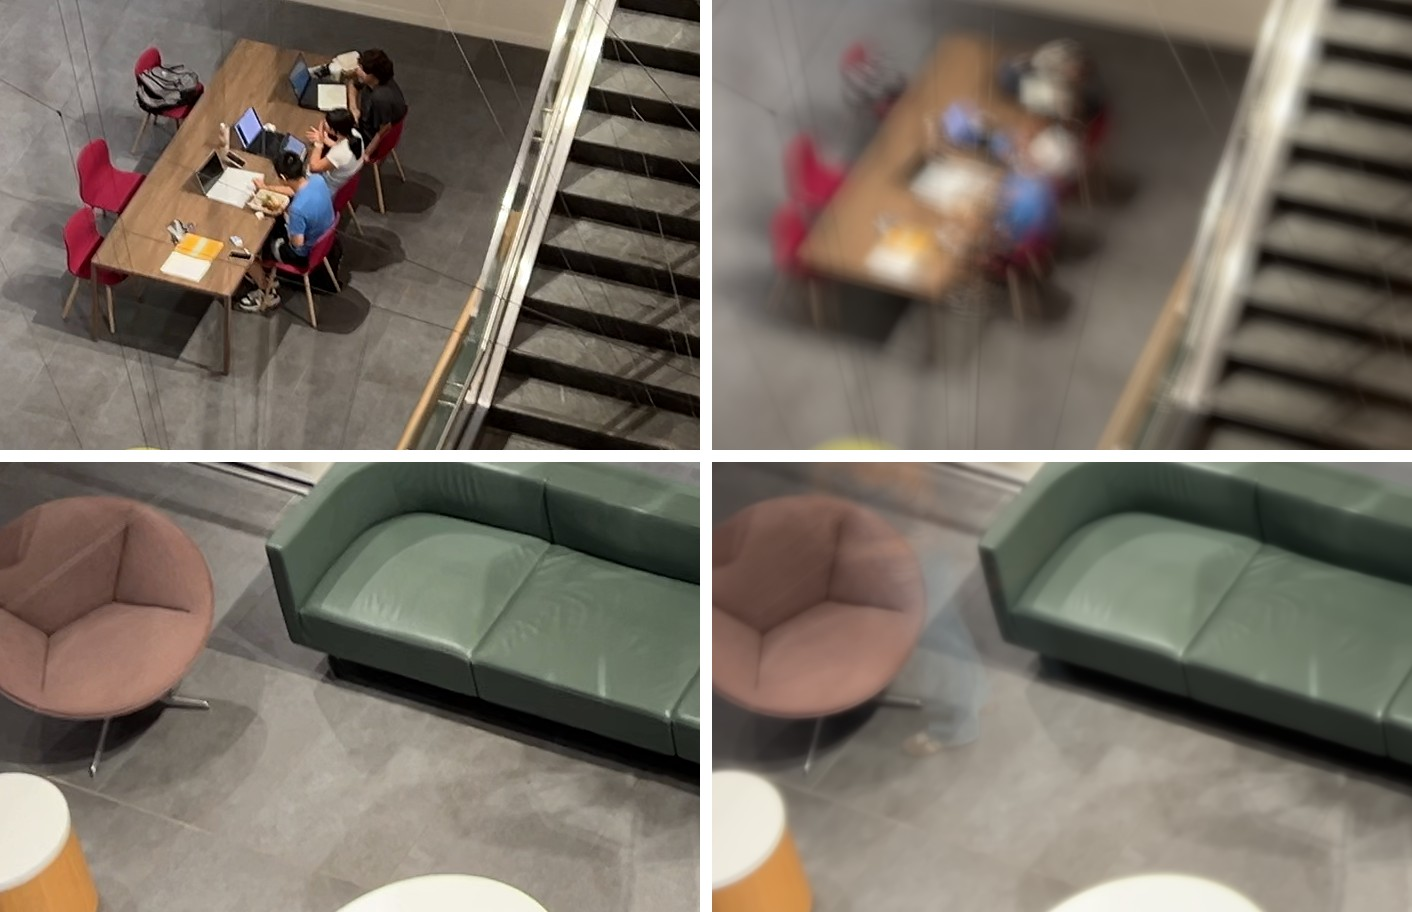
\includegraphics[width=\linewidth]{report/crops.jpg}
\caption{Full-resolution crops, reference frame left and render right. Top: the lower-floor table (predicted 33 px) is smeared into a soft disc. Bottom: the sofa on the focus plane stays sharp; a person who walked past during the sweep survives as a translucent ghost.}
\label{fig:2}
\end{figure}
\begin{figure}[htbp]
\centering

\includegraphics[width=\linewidth]{report/commons.jpg}
\caption{A second scene, the Commons dining hall, from one video and two planes. Left: tilted 38.5$^\circ$ along the floor, so tables near and far are sharp while the banners in front and the courtyard beyond blur. Right: tilted 63.5$^\circ$ the other way; the sharp band now runs across the mezzanine and the floor is out of focus.}
\label{fig:3}
\end{figure}

\section{Validation}
Before trusting real footage I rendered a synthetic city (a textured ground plane seen from above, with upright buildings) from known camera positions and ran the full pipeline on the encoded video. COLMAP recovered f = 1001 px against a true 1000 and registered all 60 frames; clicking three ground points gave a plane tilted 54.8$^\circ$ against the true 55$^\circ$. A second test renders dots at known depths by direct projection, sharing no code with the homography, and measures their rendered width: it matches $D\,f\,|1/z - 1/z_0|$ within 6 \%, and a template-matched shift-and-add of the same frames agrees with the pose-derived warp to within one grey level.

\begin{figure}[htbp]
\centering
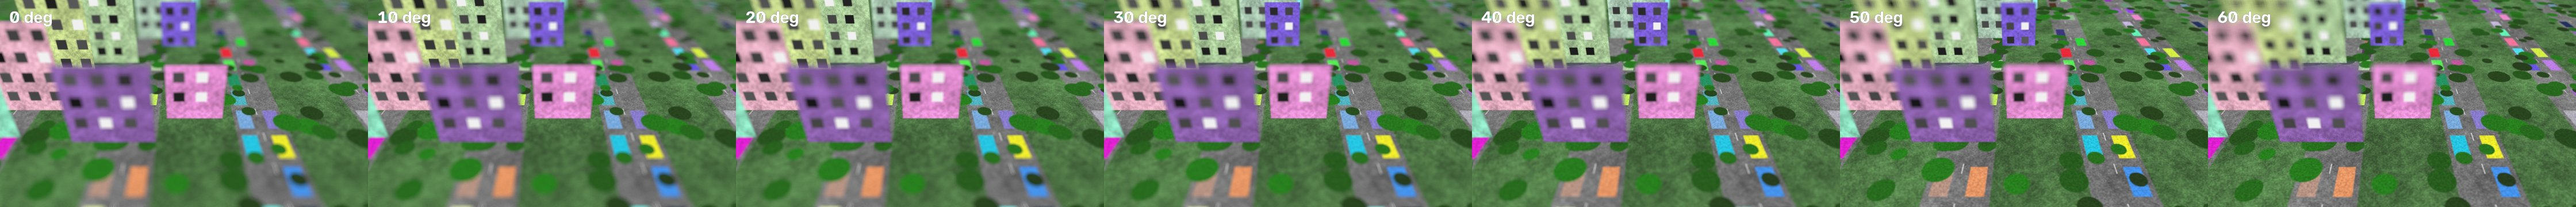
\includegraphics[width=\linewidth]{report/demo_strip.jpg}
\caption{Tilt sweep of the synthetic scene from one capture, 0$^\circ$ to 60$^\circ$, rendered in one pass over the frames.}
\label{fig:4}
\end{figure}

\section{What I learned}
\textbf{The scene decides whether the effect exists at all.} The blur at a point is $D\,f\,|1/z - 1/z_0|$: it comes from the \emph{difference} between that point's depth and the focus depth, scaled by how big the sweep is compared with the distance. A scene where everything is at nearly the same depth, like a wall seen head-on or a city skyline, produces almost no blur no matter how the plane is set, because the frames agree about everything. I tried to capture 30-60-90 from the O'Connor roof, some 50 m away, and it came out almost uniformly sharp for exactly this reason. The O'Connor lobby works because from the balcony there are objects at two metres (the column), at five (the upper-floor furniture) and at fifteen (the study table below), all in one frame. Even so, the predicted 33 px of blur on the lower floor is visible but modest; the miniature look would be stronger with a wider sweep or a nearer subject. Looking down from a height at small objects, the classic tilt-shift viewpoint, is the right choice for optical reasons, not only for the look.

\textbf{Moving people do not blur, they ghost.} A real lens takes all of its views at the same instant, so a person is at one place in every view and simply blurs if they are off the plane. My aperture is assembled over 45 seconds. Someone who walks through is at a different place in each frame, and in most frames not there at all, so the average contains a faint, transparent copy of them at each position they occupied (Figure~\ref{fig:2}, bottom right, and the diners in Figure~\ref{fig:3}).

\textbf{Focus became a decision made after the shot.} A camera normally fixes the focus at the moment of capture, and the focus plane is always the one the lens is built to give: flat and facing the camera. Here the recording stores only views. Which plane is sharp, how far it is tilted, and how wide the aperture is are all chosen afterwards, and the choice is not limited to what the pictures show, because the warp is computed from where the camera was, not from what it saw. The plane can lie along the upper floor at 26$^\circ$, or pass through the open air of the atrium, and one 45-second clip gives all of them. The cost of this freedom is that everything rests on recovering the camera positions accurately: an error in a frame's position softens the very plane that should be sharp, which is why the final image uses only the inner 80 \% of the sweep, where the positions were most reliable.


\end{document}
